\documentclass[aspectratio=169, 320mm, 180mm]{beamer}
\usepackage[utf8]{inputenc}
\usepackage{ctex}  % 提供中文支持
\usepackage{tikz}  % 使用tikz绘图
\usepackage{minted} % 使用minted高亮显示源代码
\usepackage{amsmath} % 数学公式

\usetheme{Madrid}  % 使用Madrid主题
\usecolortheme{beaver}  % 使用beaver主题颜色

% 自定义一些TikZ绘图设置
\usetikzlibrary{shapes.geometric, positioning}

\title{TikZ 绘图示例}
\author{作者}
\date{\today}

\begin{document}

\frame{\titlepage}

% 绘制点、三角形、长方形示例
\begin{frame}[fragile]{基本绘图:点、三角形、长方形}
\begin{minted}[frame=single,framesep=10pt]{latex}
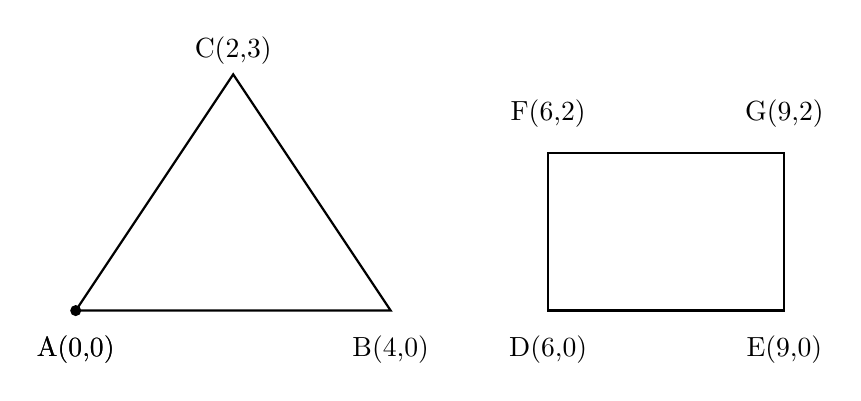
\begin{tikzpicture}
    % 画点
    \fill (0,0) circle (2pt);  % 在原点画一个小圆点
    \node at (0,-0.5) {A(0,0)};
    
    % 画三角形
    \draw[thick] (0,0) -- (4,0) -- (2,3) -- cycle;
    \node at (0,-0.5) {A(0,0)};
    \node at (4,-0.5) {B(4,0)};
    \node at (2,3.3) {C(2,3)};
    
    % 画长方形
    \draw[thick] (6,0) rectangle (9,2);
    \node at (6,-0.5) {D(6,0)};
    \node at (9,-0.5) {E(9,0)};
    \node at (6,2.5) {F(6,2)};
    \node at (9,2.5) {G(9,2)};
\end{tikzpicture}
\end{minted}
\vspace{1cm}
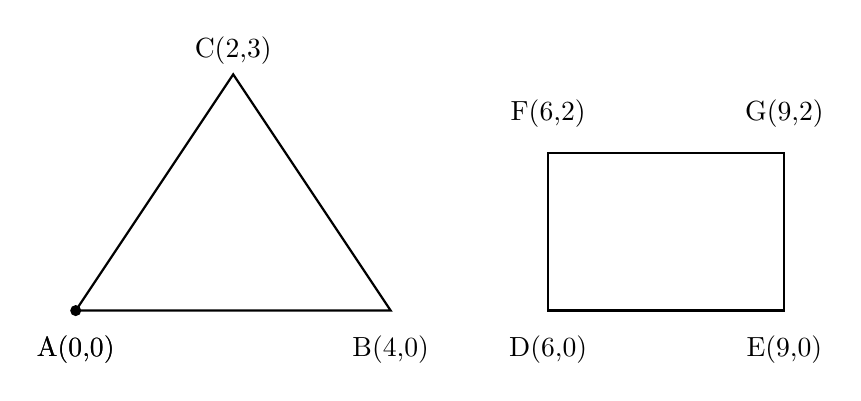
\begin{tikzpicture}
    % 画点
    \fill (0,0) circle (2pt);  % 在原点画一个小圆点
    \node at (0,-0.5) {A(0,0)};
    
    % 画三角形
    \draw[thick] (0,0) -- (4,0) -- (2,3) -- cycle;
    \node at (0,-0.5) {A(0,0)};
    \node at (4,-0.5) {B(4,0)};
    \node at (2,3.3) {C(2,3)};
    
    % 画长方形
    \draw[thick] (6,0) rectangle (9,2);
    \node at (6,-0.5) {D(6,0)};
    \node at (9,-0.5) {E(9,0)};
    \node at (6,2.5) {F(6,2)};
    \node at (9,2.5) {G(9,2)};
\end{tikzpicture}
\end{frame}

% 绘制圆、椭圆和圆弧
\begin{frame}[fragile]{基本绘图:圆、椭圆、圆弧}
\begin{minted}[frame=single,framesep=10pt]{latex}
\begin{tikzpicture}
    % 画圆
    \draw[thick] (0,0) circle (3cm);
    \node at (0,-3.5) {O(0,0)};
    
    % 画椭圆
    \draw[thick] (6,0) ellipse (3cm and 1.5cm);
    \node at (6,-2) {椭圆的中心};
    
    % 画圆弧
    \draw[thick] (9,0) arc[start angle=0, end angle=90, radius=2cm];
\end{tikzpicture}
\end{minted}
\vspace{1cm}
\begin{tikzpicture}
    % 画圆
    \draw[thick] (0,0) circle (3cm);
    \node at (0,-3.5) {O(0,0)};
    
    % 画椭圆
    \draw[thick] (6,0) ellipse (3cm and 1.5cm);
    \node at (6,-2) {椭圆的中心};
    
    % 画圆弧
    \draw[thick] (9,0) arc[start angle=0, end angle=90, radius=2cm];
\end{tikzpicture}
\end{frame}

\end{document}
